\documentclass[a4paper,12pt]{article}
%%% Русский язык
\usepackage[T2A]{fontenc}			% кодировка
\usepackage[utf8]{inputenc}			% кодировка исходного текста
\usepackage[english,russian]{babel}	% локализация и переносы
\usepackage{indentfirst}
\frenchspacing

\renewcommand*{\epsilon}{\ensuremath{\varepsilon}}
\renewcommand*{\phi}{\ensuremath{\varphi}}
\renewcommand*{\kappa}{\ensuremath{\varkappa}}
\renewcommand*{\le}{\ensuremath{\leqslant}}
\renewcommand*{\leq}{\ensuremath{\leqslant}}
\renewcommand*{\ge}{\ensuremath{\geqslant}}
\renewcommand*{\geq}{\ensuremath{\geqslant}}
\renewcommand*{\emptyset}{\varnothing}

%% Перенос знаков в формулах (по Львовскому)
\newcommand*{\hm}[1]{#1\nobreak\discretionary{}
{\hbox{$\mathsurround=0pt #1$}}{}}

%%% Tables
\usepackage{array,tabularx,tabulary,booktabs}
\usepackage{longtable}
\usepackage{multirow}

%%% Images
\usepackage{graphicx}
\graphicspath{{images/}{images2/}}
\setlength\fboxsep{3pt}
\setlength\fboxrule{1pt}
\usepackage{wrapfig}
\usepackage{tikz}
\usepackage{pgfplots}
\usepackage{pgfplotstable}

%%% AMS
\usepackage{amsmath,amsfonts,amssymb,amsthm,mathtools}
\usepackage{icomma}

%%% Fields
\usepackage{geometry}
% \geometry{top=25mm}
% \geometry{bottom=35mm}
% \geometry{left=35mm}
% \geometry{right=20mm}

%%% Making the bibliography appear in the table of contents
%%% https://tex.stackexchange.com/questions/8458/making-the-bibliography-appear-in-the-table-of-contents
\usepackage[nottoc]{tocbibind}

%%% Diff
\usepackage{cmap} % Search in PDF
\usepackage{mathtext}
\usepackage{xspace}
\usepackage{etoolbox} % Logical operators
\usepackage{listings}
\usepackage{color}
\usepackage{lastpage}
\usepackage{soul}
\usepackage{hyperref}
%\usepackage[usenames,dvipsnames,svgnames,table,rgb]{xcolor}
\usepackage{csquotes}
\usepackage{multicol}
\usepackage{array}
\usepackage{setspace}
\newcolumntype{L}[1]{>{\raggedright\let\newline\\\arraybackslash\hspace{0pt}}m{#1}}
\newcolumntype{C}[1]{>{\centering\let\newline\\\arraybackslash\hspace{0pt}}m{#1}}
\newcolumntype{R}[1]{>{\raggedleft\let\newline\\\arraybackslash\hspace{0pt}}m{#1}}

\definecolor{mygreen}{rgb}{0,0.6,0}
\definecolor{mygray}{rgb}{0.5,0.5,0.5}
\definecolor{mymauve}{rgb}{0.58,0,0.82}

\lstset{
  frame=none,
  xleftmargin=2pt,
  stepnumber=1,
  numbers=left,
  numbersep=5pt,
  numberstyle=\ttfamily\scriptsize\color[gray]{0.3},
  belowcaptionskip=\bigskipamount,
  captionpos=b,
  escapeinside={*'}{'*},
  language=haskell,
  tabsize=2,
  emphstyle={\bf},
  commentstyle=\it,
  stringstyle=\mdseries\rmfamily,
  showspaces=false,
  keywordstyle=\bfseries\rmfamily,
%   columns=flexible,
  basicstyle=\small\ttfamily,
  showstringspaces=false,
  morecomment=[l]\%,
  breaklines,
  columns=fullflexible,
  flexiblecolumns,
  numbers=left,
  numberstyle={\footnotesize},
  extendedchars=\true,
  keepspaces=true,
}

% \lstset{
%   backgroundcolor=\color{white},   % choose the background color; you must add \usepackage{color} or \usepackage{xcolor}; should come as last argument
%   basicstyle=\footnotesize,        % the size of the fonts that are used for the code
%   breakatwhitespace=false,         % sets if automatic breaks should only happen at whitespace
%   %breaklines=true,                 % sets automatic line breaking
%   captionpos=с,                    % sets the caption-position to bottom
%   commentstyle=\color{mygreen},    % comment style
%   deletekeywords={...},            % if you want to delete keywords from the given language
%   escapeinside={\%*}{*)},          % if you want to add LaTeX within your code
%   extendedchars=true,              % lets you use non-ASCII characters; for 8-bits encodings only, does not work with UTF-8
%   %firstnumber=1000,                % start line enumeration with line 1000
%   %frame=single,	                   % adds a frame around the code
%   keepspaces=true,                 % keeps spaces in text, useful for keeping indentation of code (possibly needs columns=flexible)
%   %keywordstyle=\color{blue},       % keyword style
%   %language=SQL,                 % the language of the code
%   %morekeywords={*,...},            % if you want to add more keywords to the set
%   %numbers=left,                    % where to put the line-numbers; possible values are (none, left, right)
%   %numbersep=5pt,                   % how far the line-numbers are from the code
%   %numberstyle=\tiny\color{mygray}, % the style that is used for the line-numbers
%   rulecolor=\color{black},         % if not set, the frame-color may be changed on line-breaks within not-black text (e.g. comments (green here))
%   showspaces=false,                % show spaces everywhere adding particular underscores; it overrides 'showstringspaces'
%   showstringspaces=false,          % underline spaces within strings only
%   showtabs=false,                  % show tabs within strings adding particular underscores
%   stepnumber=2,                    % the step between two line-numbers. If it's 1, each line will be numbered
%   stringstyle=\color{mymauve},     % string literal style
%   tabsize=2,	                   % sets default tabsize to 2 spaces
%   title=\lstname                   % show the filename of files included with \lstinputlisting; also try caption instead of title
% }

\mathtoolsset{showonlyrefs=true} % Numerete only formules with references

\newcommand*{\yooline}[1]{\overline{\overline{#1}}}
\newcommand*{\yeqdef}{\overset{\underset{\mathrm{def}}{}}{=}}
\newcommand*{\Pn}{\ensuremath{\mathbf{P}^n}}
\newcommand*{\R}{\ensuremath{\mathbb R}\xspace}
\newcommand*{\Laplace}{\mathop{}\!\mathbin\bigtriangleup}
\newcommand*{\DAlambert}{\mathop{}\!\mathbin\Box}
\DeclareMathOperator{\sgn}{\mathop{sgn}}

%% VsCode liter suggested to add
\pgfplotsset{compat=1.17}



\begin{document}

\thispagestyle{empty}
\begin{center}
    Computer Science Center

    Yandex ML \& Data Management Lab
\end{center}
\vspace{13ex}

\begin{center}
    \vspace{16ex}
    \begin{spacing}{1.5}
        {\Large Контрактное программирование \\как способ задания и оптимизации вычислительных графов для распределённых потоковых систем}
    \end{spacing}
\end{center}
\vfill
\begin{flushright}
    \noindent
    \textit{Руководитель: Трофимов Артём} \\
    \textit{Студент: Стоян Андрей}
\end{flushright}
\vspace{5ex}
\begin{center}
    СПб 2020
\end{center}
\newpage

\tableofcontents
\newpage

\section{Введение}

Приложения, обрабатывающие большие объёмы данных, используют фраемворки, позволяющие производить вычисления с состоянием над ограниченными и неограниченными потоками данных, такие как, например, Apache Flink \cite{flink-org}.

Такие фраемворки обычно запускаются на кластере машин, получают запросы на обработку данных от приложений и могут отправлять результат назад в приложение, складывать в базу данных, формировать новый поток данных для последующей обработки и т.д. (см. рис. \ref{fig:flink-app}).

\begin{figure}[h]
    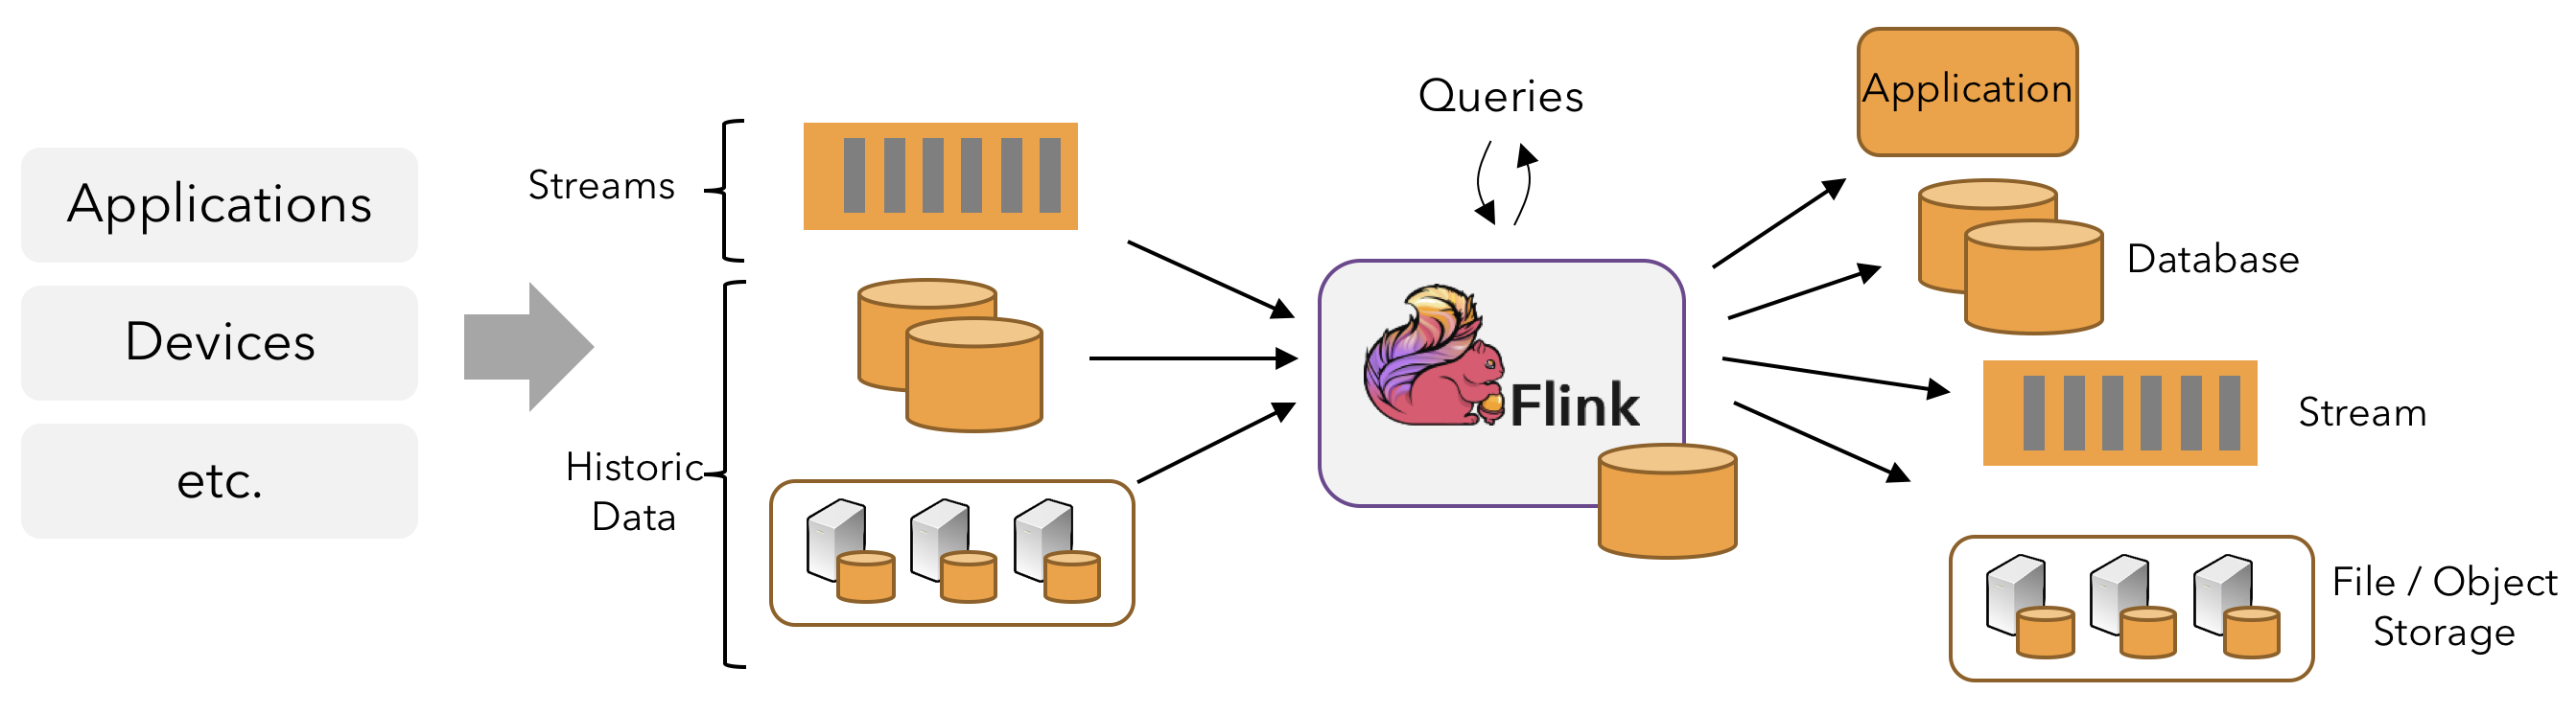
\includegraphics[width=\textwidth]{flink-app.png}
    \caption{Использование Apache Flink.}
    \label{fig:flink-app}
\end{figure}

Запросы формируются в виде вычислительного графа (пайплайна), который представляет собой ориентированный граф без циклов. Пример задания такого графа представлен на рисунке \ref{fig:prog-data}.

\begin{figure}
    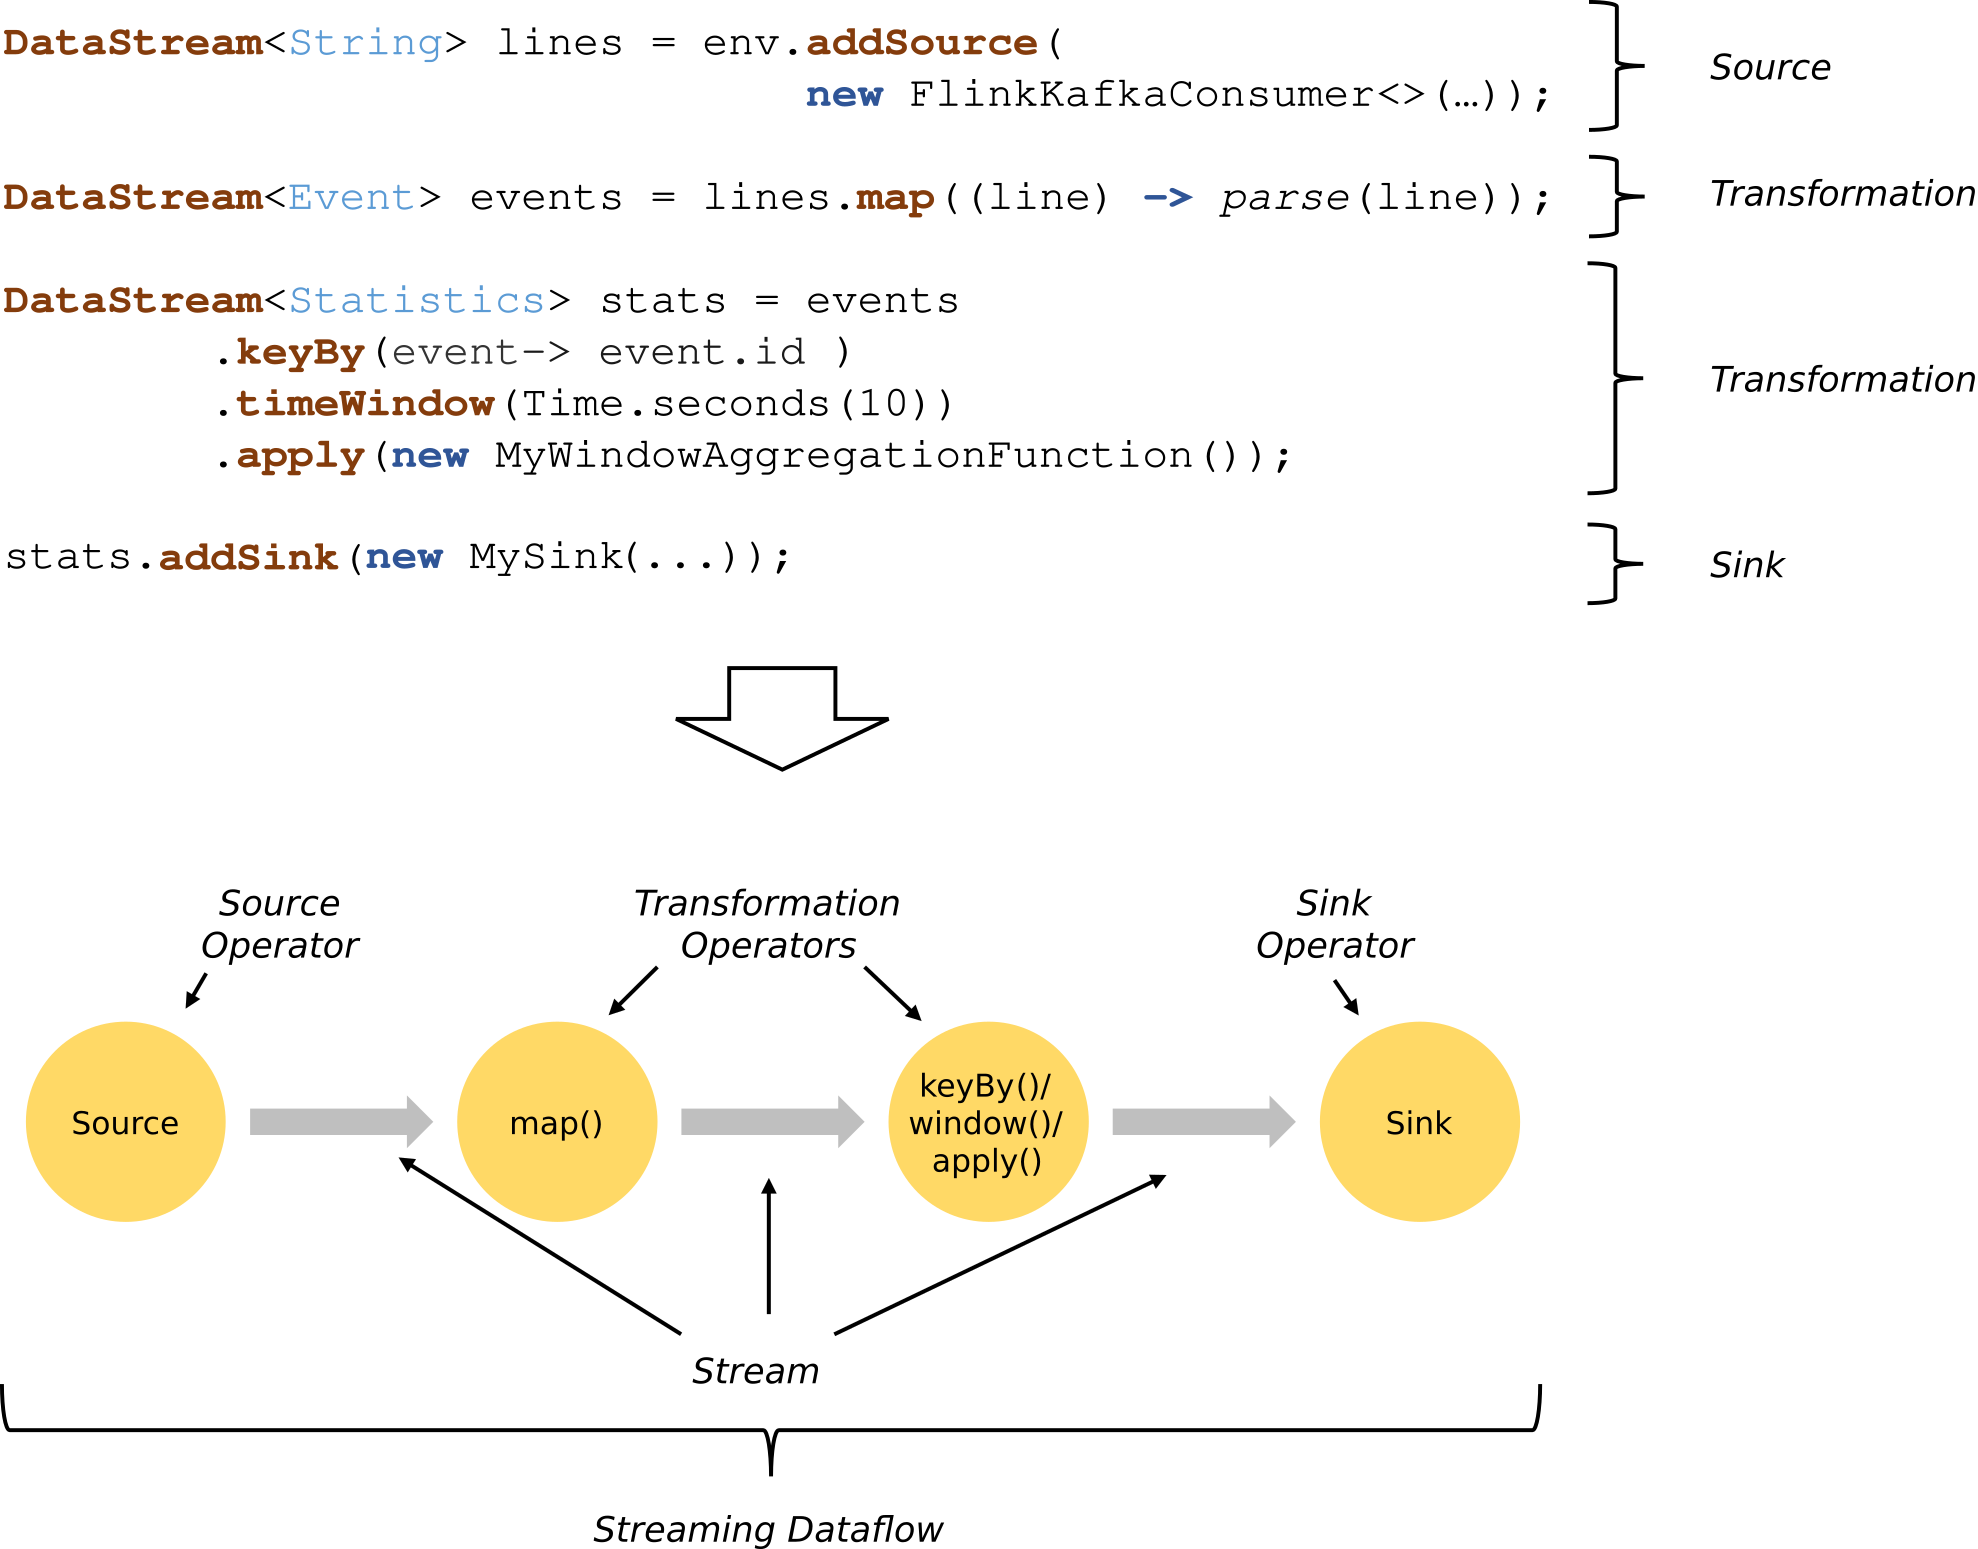
\includegraphics[width=\textwidth]{program_dataflow.png}
    \caption{Пример вычислительного графа для Apache Flink.}
    \label{fig:prog-data}
\end{figure}

Копии пайплайна распределяются между машинами для параллельной обработки данных.
Часть операций не содержат состояния и не требуют дополнительных усилий, чтобы быть запущенными в нескольких экземплярах, и работать параллельно.
Некоторые операции же, такие как агрегация, требуют наличия изменяемого состояния и требуют специального перераспределения (решардирования) данных между их экземплярами. Пример показан на рисунке \ref{fig:par-data}.

\begin{figure}
    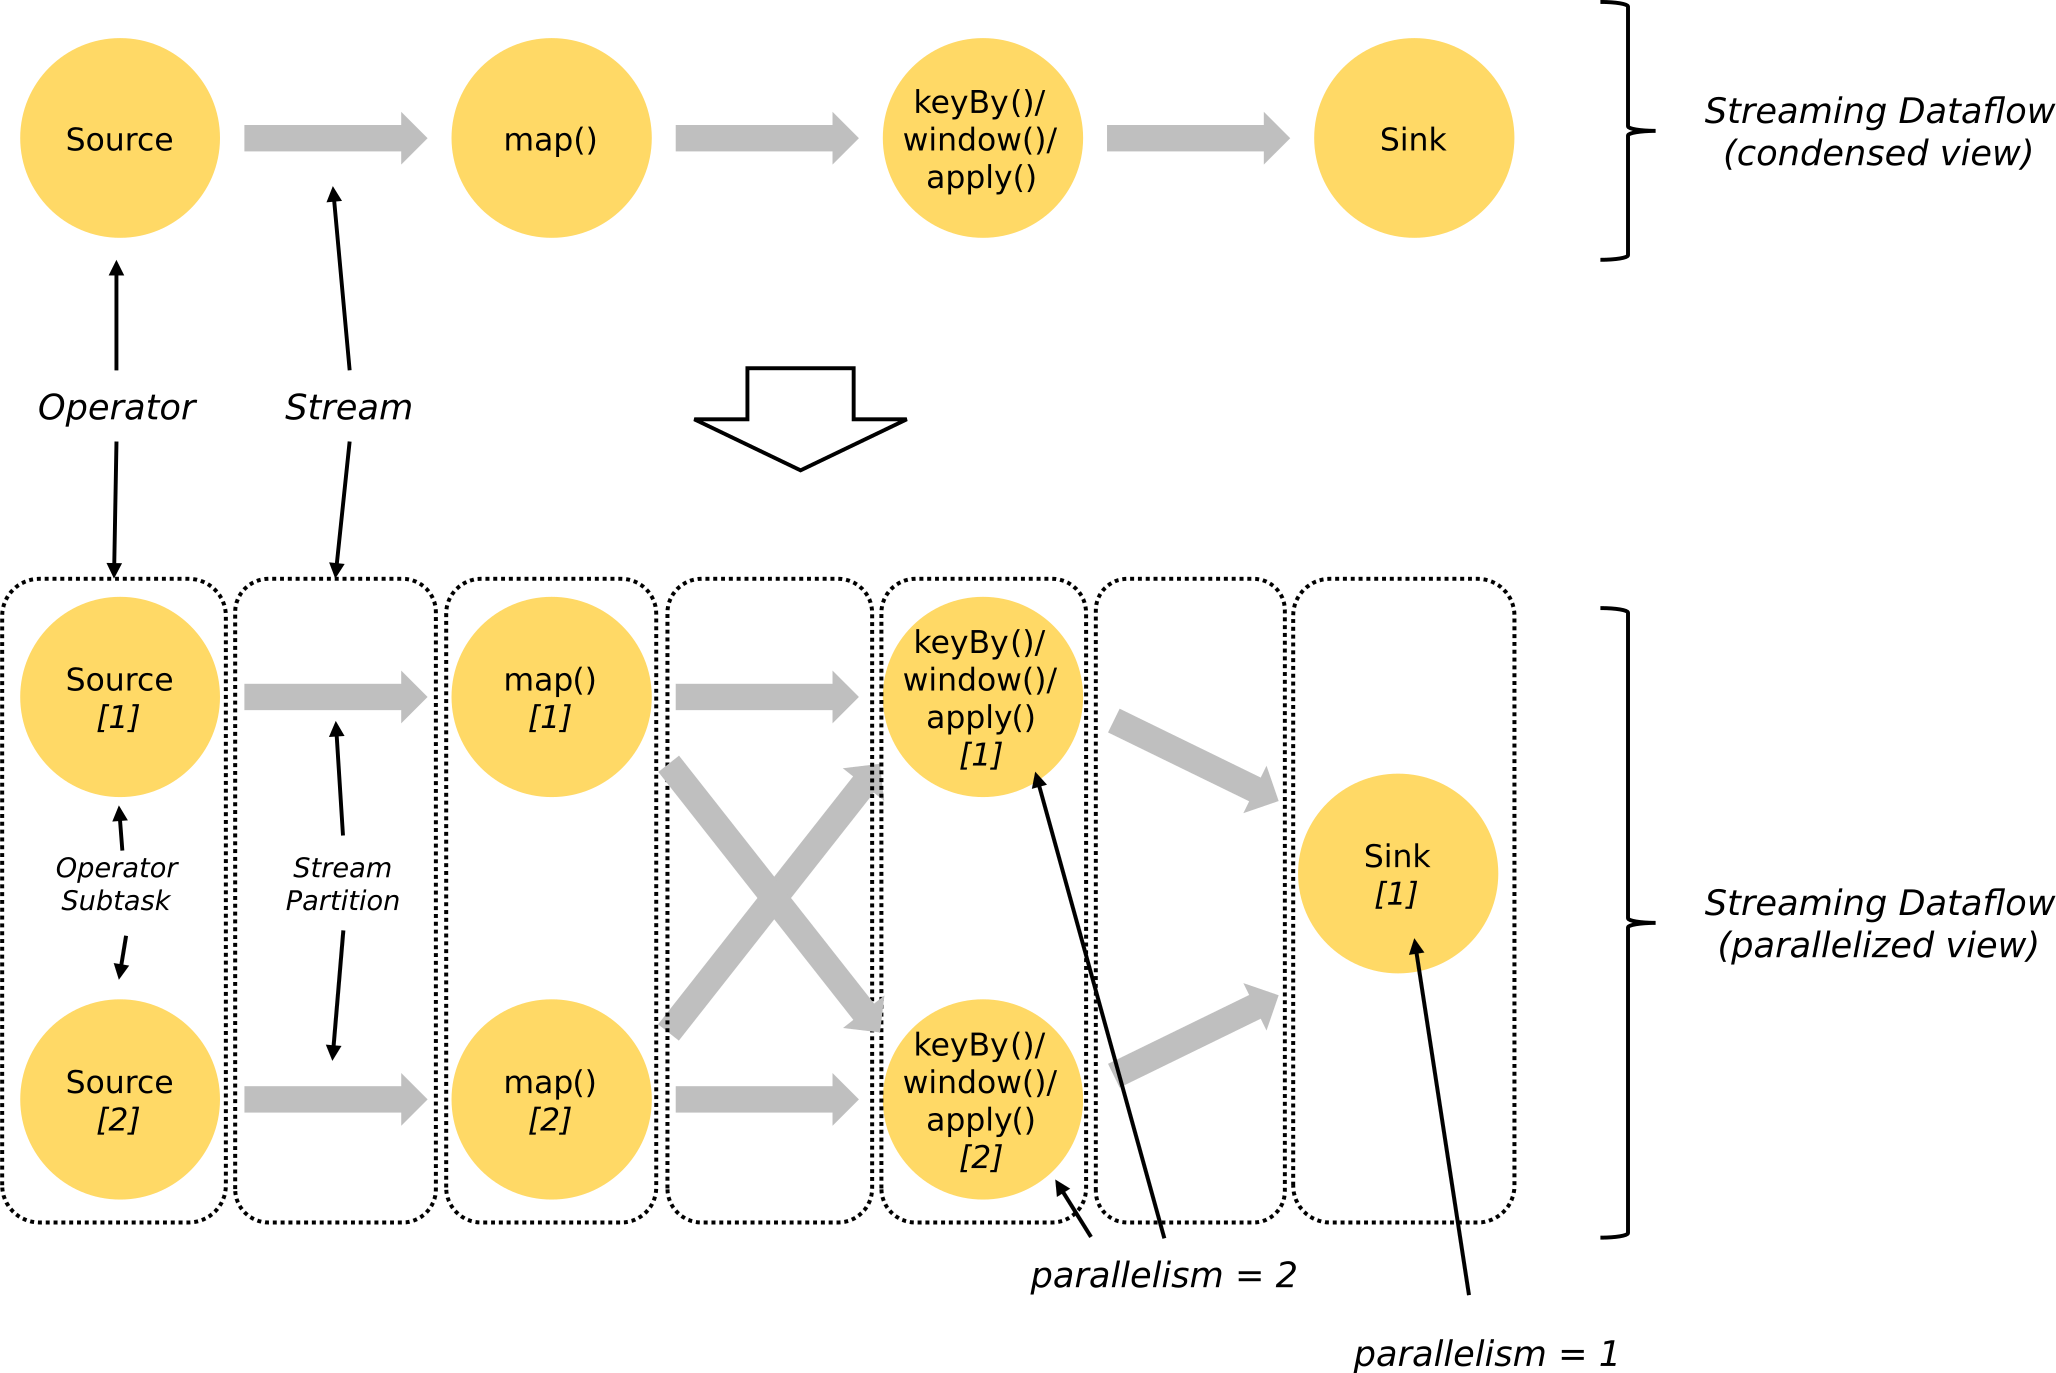
\includegraphics[width=\textwidth]{parallel_dataflow.png}
    \caption{Распределение данных между экземплярами операций одного и того же пайплайна, размещёнными на разных машиных. Операция \textit{map()} не имеет состояния, и её два экземпляра параллельно обрабатывают один и тот же поток данных, не влияя друг на друга. Операция \textit{apply()} же имеет изменяемое состояние, поэтому необходимо производить перераспределение данных (решардирование) между её экземплярами с помощью \textit{keyBy()}.}
    \label{fig:par-data}
\end{figure}

В данной работе предлагается новый способ задания вычислительных графов для распределённых потоковых систем, который позволяет упростить программирование комплексных пайплайнов и производить их автоматическую оптимизацию.

Все материалы работы можно найти в \href{https://github.com/winter-yuki/calco}{GitHub репозитории проекта}.

\newpage
\section{Проблема}

Современные фреймворки предоставляют два основных способа задания графов: композиция примитивных операций (\textit{Map}, \textit{Reduce} и т.д.) и SQL запросы (диалект Streaming SQL, для потоковой обработки \cite{streaming-sql}). На рисунке \ref{fig:api-stack} представлена иерархия  Apache Flink API.

\begin{figure}[h]
    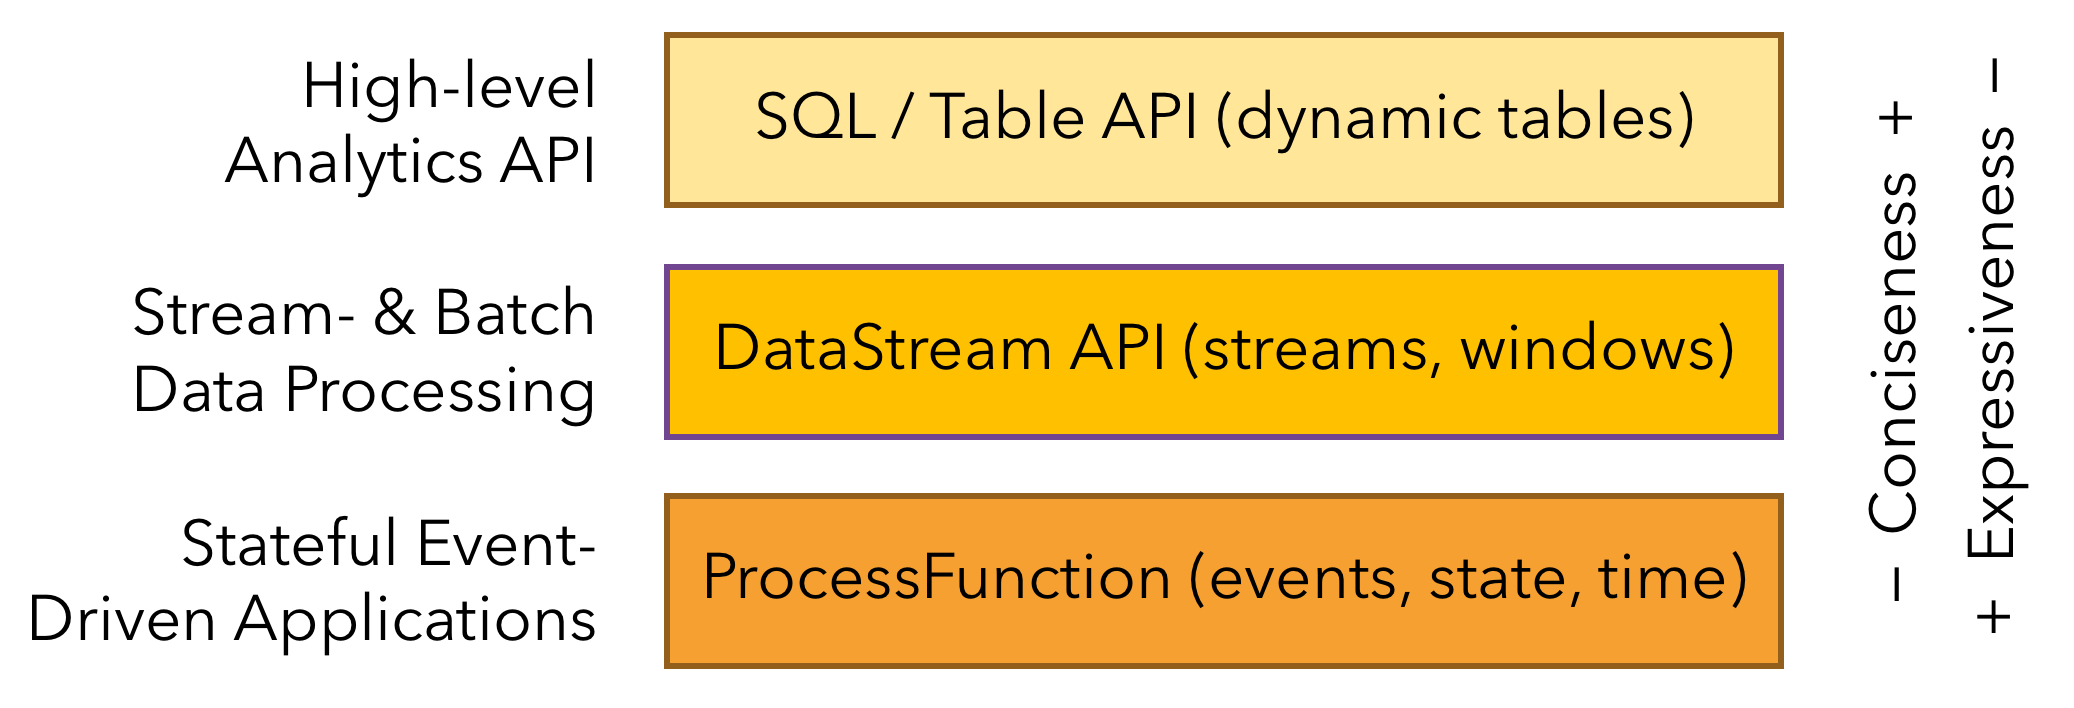
\includegraphics[width=\linewidth]{api-stack.png}
    \caption{Иерархия Apache Flink API. Видим, что фреймворк предоставляет три уровня интерфейсов: от самого выразительного, \textit{ProcessFunction}, до самого лаконичного, SQL. \textit{ProcessFunction} и \textit{DataStream} позволяют определять операции и составлять их композиции.}
    \label{fig:api-stack}
\end{figure}

Пусть мы хотим записать граф, схематично изображенный на рисунке \ref{fig:complex-graph}.

\begin{figure}[h]
    \centering
    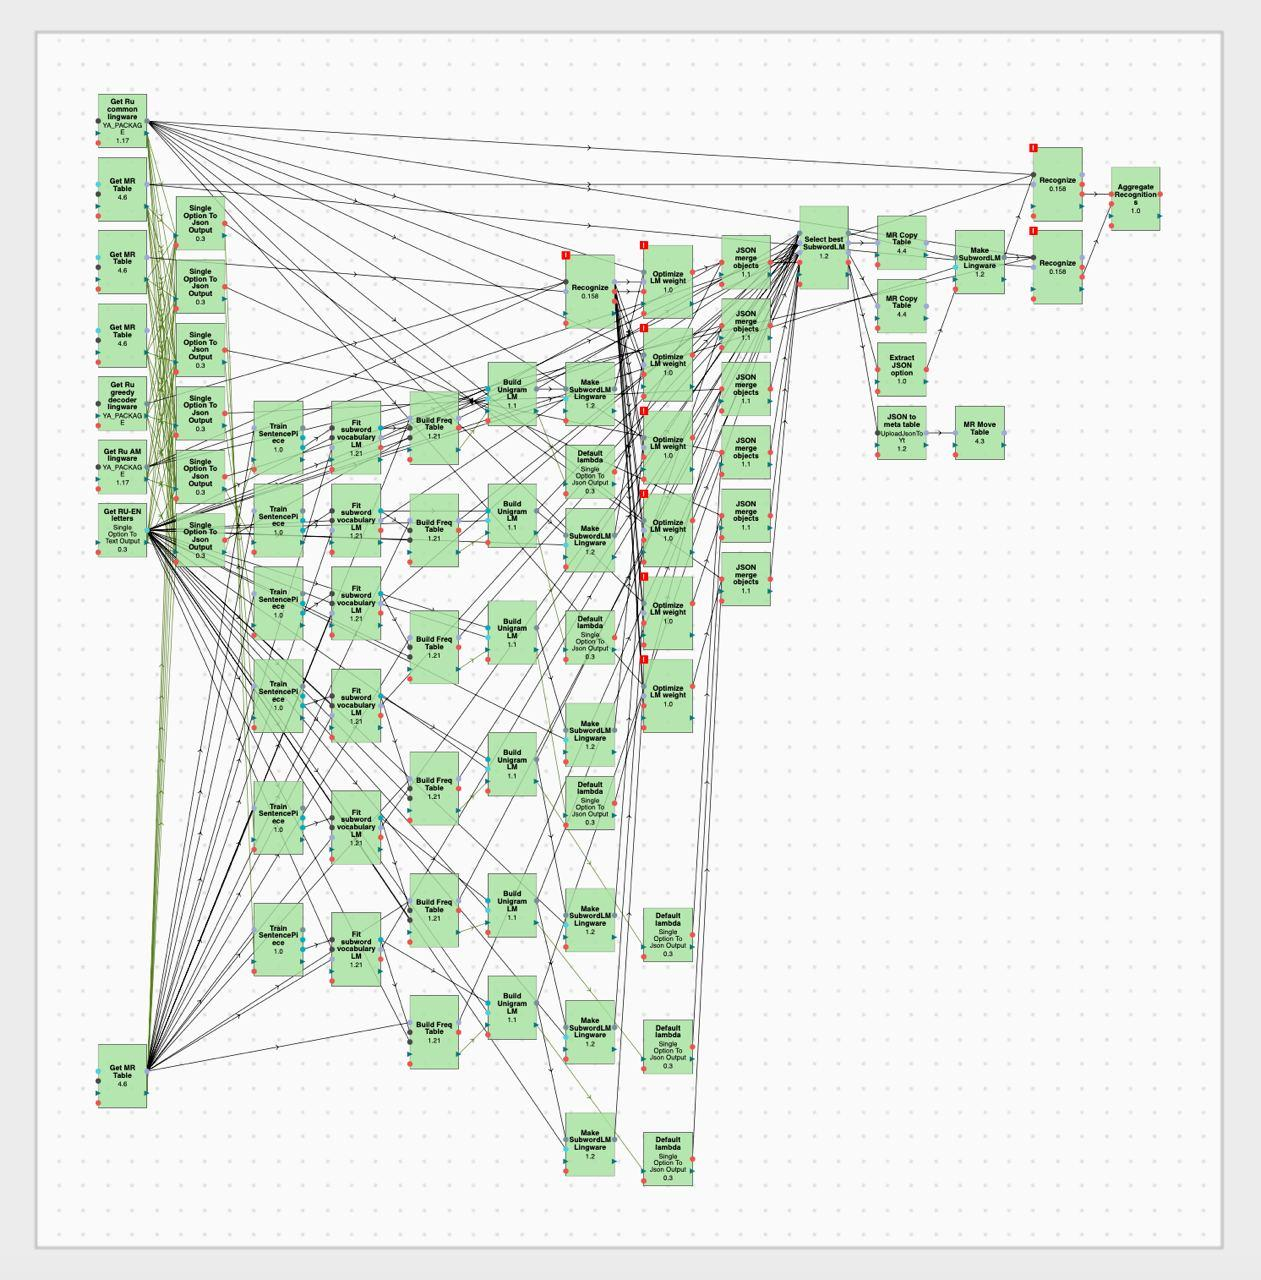
\includegraphics[width=0.8\linewidth]{complex-graph.jpg}
    \caption{Графы, производящие обработку данных для реальных приложений могут быть довольно большими.}
    \label{fig:complex-graph}
\end{figure}

Когда мы составляем граф как композицию операций (как на рисунке \ref{fig:prog-data}),
мы однозначно определяем их порядок и не предоставляем фреймворку информации о том,
какие операции с какими можно переставлять в целях оптимизации, оставляя пайплайн корректным.
Таким образом, возможна только ручная оптимизация.

Диалект Streaming SQL позволяет использовать в SQL запросах неограниченные источники данных.
Как и в случае с традиционным SQL, он предназначен для выборки данных из источников и подсчёта статистик, а не для записи комплексной бизнес-логики.

Пусть мы уже имеем написанный и работающий на кластере граф \ref{fig:complex-graph}.
Попробуем добавить этому графу ещё одну функциональность и вернуть на кластер.
Постараемся максимально использовать промежуточные значения, вычисленные в исходном графе, чтобы не производить лишних повторных вычислений.

Сейчас для таких модификаций требуется вручную исправлять граф и производить оптимизации (минимизировать количество решардирований, размещать фильтрации как можно ближе к источникам данных и т.д.). В случае больших графов это довольно сложная работа, подверженная трудно уловимым ошибкам.

Таким образом, требуется разработать декларативный подход к описанию вычислительных графов, который бы упростил их задание и модификацию, и позволил бы производить автоматические оптимизации путём перестановки операций в графе.

\newpage
\section{Идея}

Вершины вычислительных графов могут быть двух типов: \textbf{источники} и операции (\textbf{трансформации}). Источники не получают данных, только отдают. Операции принимают один или несколько потоков данных и могут порождать поток данных, а так же могут формировать результаты работы графа (в виде записи в базе данных, нового потока для другой системы, и т.д.).

Будем называть \textbf{нодами} вершины обоих типов.

Чтобы иметь возможность изменять форму графа, для каждой операции необходимо иметь информацию о требованиях, которые она выдвигает к данным, поступающим на её вход, и гарантии, которые она выставляет для производимых ею данных.

Такие требования и гарантии назовём \textbf{контрактами} операции, \textbf{входными} и \textbf{выходными} соответственно.

Далее будут приводиться листинги на языке Haskell, формализующие вводимые понятия.

\begin{lstlisting}
    -- InCont - входной контракт.
    -- OutCont - выходной контракт.
    -- Пока предположим, что трансформаций арности два будет достаточно.

    -- Вершины вычислительного графа, аннотированные контрактами
    data Node =
        Stream OutCont             -- Источник данных.
      | Tfm1 InCont OutCont        -- Трансформация арности один.
      | Tfm2 InCont InCont OutCont -- Трансформация арности два.
\end{lstlisting}

Зададим множество нод, аннотированных контрактами (\textbf{окружение}):
\begin{lstlisting}
    type Env = Map NodeName Node
\end{lstlisting}

Определим \textbf{семантику} вычислительного графа как подмножество множества нод, элементы которого формируют требуемые от графа результаты работы:
\begin{lstlisting}
    type Semantics = Set NodeName
\end{lstlisting}

Наконец, определим \textbf{ц-граф}, который перставляет собой пару из окружения и семантики:
\begin{lstlisting}
    type CGraph = (Env, Semantics)
\end{lstlisting}

Пусть ц-граф задаёт множество \textbf{конкретных графов} (или просто \textbf{графов}) следующим образом:
граф задаётся данным ц-графом, если он состоит только из нод окружения, содержит каждую ноду семантики один раз, и контракты всех используемых нод удовлетворяются.

Будем использовать ц-графы в качестве нового способа задания вычислительных графов.
Каждый конкретный граф содержит ноды, формирующие требуемый результат работы.
Все ноды каждого графа получают валидные данные на вход и, следовательно, работают корректно.
Таким образом, все операции семантики так же работают корректно, и каждый граф, соответствующий данному ц-графу, выполняет одну и ту же, требуемую, работу.

Процесс от задания ц-графа до запуска задачи на целевом фреймворке выглядит следующим образом:
\begin{lstlisting}
    -- [Graph] - список графов.
    -- Точка - оператор композиции функций.

    -- RGraph - конкретный граф в API целевого фреймворка.
    run :: CGraph -> Runtime RGraph
    run = graphToRGraph    -- Преобразовать конкретный граф в
                           -- вычислительный граф целевого фреймворка.
        . chooseGraph cost -- Выбрать оптимальный граф в соответствии
                           -- с функцией оценки cost.
        . genGraphs        -- Сгенерировать все графы, соответствующие
                           -- данному CGraph.

    genGraphs :: CGraph -> [Graph]
    cost :: Graph -> Integer
    chooseGraph :: (Graph -> Integer) -> [Graph] -> Graph
    graphToRGraph :: Graph -> Runtime RGraph
\end{lstlisting}


\subsection{Конкретные графы}

Будем представлять граф виде множества термов. Результат работы одной ноды может подаваться на вход нескольким нодам, поэтому в операциях будем хранить не сами подтермы, а их идентификаторы.

\begin{lstlisting}
    data Term =
        Const NodeName
      | App1 NodeName TermId
      | App2 NodeName TermId TermId

    type Graph = Map TermId Term
\end{lstlisting}


\subsection{Контракты}

Будем считать, что данные имеют формат записей с именованными атрибутами.
Тогда существует два сорта информации о потоке данных: какие атрибуты имеют записи и какие существуют свойства атрибутов и связей между ними.

Введём состояние потока как совокупность информации о нём:
\begin{lstlisting}
    -- Атрибуты
    type Attr = AttrName

    -- Свойства
    type Prop = PropName

    data Scheme = Scheme
      { attrs :: Set Attr -- Множество атрибутов в потоке.
      , props :: Set Prop -- Множество свойств в потоке.
      }
\end{lstlisting}

Введём входной контракт и правило проверки:
\begin{lstlisting}
    data InCont = InCont
      { attrsI  :: Set Attr -- Множество требуемых атрибутов.
      , propsI  :: Set Prop -- Множество требуемых свойств.
      , propsI' :: Set Prop -- Множество запрещённых свойств.
      }

    match :: Scheme -> InCont -> Bool
    match s c = attrsI c `Set.isSubsetOf` attrs s
             && propsI c `Set.isSubsetOf` props s
             && propsI' c `Set.disjoint`  props s
\end{lstlisting}

Пусть выходной контракт определяет разницу между состояниями входного и выходного потоков. Введём выходной контракт и правило обновления состояния:

\begin{lstlisting}
    data OutAttrs =
        AddAttrs (Set Attr) -- К множеству входящих атрибутов
                            -- добавятся новые из множества.
      | NewAttrs (Set Attr) -- Множество входящих атрибутов
                            -- заменится на новое.

    data OutCont = OutCont
      { attrsO  :: OutAttrs -- Изменения в составе атрибутов
                            -- относительно требуемых.
      , propsO  :: Set Prop -- Множество добавляемых свойств.
      , propsO' :: Set Prop -- Множество удаляемых свойств.
      }

    update :: Scheme -> OutCont -> Scheme
    update s c =
      Scheme { attrs = attrs'
            , props = propsO c `Set.union' (props s \\ propsO' c) }
      where
        attrs' = case attrsO c of
          AddAttrs attrs' -> attrs' `Set.union' attrs s
          NewAttrs attrs' -> attrs'
\end{lstlisting}

Если если в операцию входят два потока, то чтобы посчитать состояние выхода, состояния входных потоков объединяются:

\begin{lstlisting}
    union :: Scheme -> Scheme -> Scheme
    union s1 s2 = Scheme { attrs = attrs s1 `Set.union` attrs s2
                        , props = props s1 `Set.union` props s2 }
\end{lstlisting}

Cостояние ребра, выходящего из источника совпадают с выходным контрактом этого источника. Если состояние входящих рёбер удовлетворяет входным контрактам операции, то состояние выходящих вычисляется обновлением состояния входа в соответствии с выходным контрактом.

Таким образом, мы умеем для конкретного графа вычислять состояния всех его рёбер и проверять контракты всех его нод.


\subsection{Верификация}

Заметим, что предложенная система контрактов является также и средством верификации вычислительных графов, подобным логике Хоара, предназначенной для доказательства корректности императивных компьютерных программ. В логике Хоара задаются так называемые тройки Хоара~--- предусловие, команда и постусловие. Программа считается корректной, если удовлетворяются предусловия и постусловия \cite{hoare}.

\newpage
\section{Вид реализации}

Реализация состоит из двух частей: основная, которую предполагается использовать на практике, и прототип, представляющий собой высокоуровневое описание модели контрактов и работы с ней.

\subsection{Основная реализация}

Основная реализация представлена в виде библиотеки на языке Python, позволяющей использовать ц-графы для задания вычислительных графов в Apache Beam Python API \cite{beam-py}.

Проект Apache Beam предоставляет универсальную модель задания вычислительных графов и позволяет запускать графы, написанные в этой модели, в различных рантаймах \cite{beam}. Например, на Apache Flink, который мы в качестве примера рассматривали выше.

Python был выбран как язык с динамической типизацией, потому что статическая мешала бы произвольной перестановке пользовательских операций.

Реализацию библиотеки можно найти в \href{https://github.com/flame-stream/calco/tree/master/calco}{GitHub репозитории}.

\subsection{Прототип}

Для реализации прототипа был выбран Haskell~--- чистый функциональный язык программирования с сильной статической системой типов.

В терминах типов удобно вводить нужные нам понятия, что и было сделано выше.
Статическая типизация предоставляет довольно высокие гарантии корректности.
А выразительность функционального языка позволяет естественно и довольно формально описывать работу с контрактами.

В прототипе не предполагалось реализовывать тела операций, аннотированных контрактами, поэтому статическая типизация не является проблемой в данном случае.

Реализацию прототипа можно найти в \href{https://github.com/flame-stream/calco/tree/master/calcohs}{GitHub репозитории проекта}.

\newpage
\section{Предварительные результаты}

TODO Предварительные результаты

\section{Дальнейшая работа}

Несмотря на объём проделанной работы, реализуемость идеи ещё не доказана:
\begin{itemize}
    \setlength\itemsep{-0.2em}
    \item Не очевидно существование достаточно быстрого алгоритма перебора всех конкретных графов, задаваемых данным ц-графом. Ожидается, что много вариантов будут отсеиваться как не удовлетворяющие контрактам, и большая асимптотика переборного алгоритма не будет сказываться на практике.
    \item В основной реализации требуется предоставить универсальный доступ к именованным атрибутам записей для кода пользовательских операций, аннотированных контрактами. Но ключевые операции Apache Beam нередко принимают и возвращают довольно комплексные структуры данных, для которых сложно обеспечить требуемое API \cite{beam-transforms}.
\end{itemize}

До применения ц-графов на практике требуется ещё решить следующие задачи:
\begin{itemize}
    \setlength\itemsep{-0.2em}
    \item Рассмотреть большое количество примеров из практики, поправить контракты и способ их записи, чтобы удобно было решать практические задачи.
    \item Перенести реализацию с прототипа на Python.
    \item Разработать функцию оценки, чтобы в соответствии с ней выбирать самый оптимальный конкретный граф.
\end{itemize}

\section{Вывод}

TODO conclusion

\section*{Приложение А: развитие идеи}
\addcontentsline{toc}{section}{Приложение А: развитие идеи}

Первоначальной идеей была следующая: задавать множество графов, решающих данную задачу как пару из типа требуемого результата вычислений и набора типизированных функций (операций) и констант (потоков)~--- контекста.
Тогда каждый конкретный граф задавался бы термом, имеющим заданный тип в данном контексте.
Имея алгоритм, перебирающий такие термы, мы бы получали множество конкретных графов, решающих нашу задачу.
При наличии функции оценки эффективности конкретного графа, можно было бы выбрать из множества самый эффективный.

Этот подход позволяет в задании пайплайна абстрагироваться от конкретных топологий графов, не указывая конкретные потоки данных.

Существует попытка реализации этого подхода: \url{https://github.com/solariq/yasm4u}.

TODO appendix A


\begin{thebibliography}{9}
    \bibitem{flink-org} Apache Flink: \url{https://flink.apache.org/}.
    \bibitem{streaming-sql} Реализация диалекта Streaming SQL в Apache Calcite: \url{https://calcite.apache.org/docs/stream.html}.
    \bibitem{beam} Apache Beam: \url{https://beam.apache.org/}.
    \bibitem{beam-py} Apache Beam Python API: \url{https://beam.apache.org/documentation/sdks/python/}.
    \bibitem{beam-transforms} Core Beam transforms: \url{https://beam.apache.org/documentation/programming-guide/#core-beam-transforms}.
    \bibitem{rowpoly} Gaster, Benedict R., and Mark P. Jones. A polymorphic type system for extensible records and variants. Technical Report NOTTCS-TR-96-3, Department of Computer Science, University of Nottingham, 1996.
    \bibitem{hoare} Hoare logic: \url{https://en.wikipedia.org/wiki/Hoare_logic}.
\end{thebibliography}

\end{document}
